
\chapter{Clickbaits und die Klassifizierung von Clickbaits}\label{ch4}


Clickbaits besitzen semantische und syntaktische Eigenschaften, auf die besonders vorgegangen werden muss. Dies geschieht in Form von Analyse und Vorverarbeitung. In diesem Abschnitt werden Ansätze aus der Literatur verglichen, die diese semantischen und syntaktischen Besonderheiten bearbeiten. Die Ansätze aus der Literatur, haben die Oberaufgabe Clickbaits zu Klassifizieren. Damit entstehen Unteraufgaben wie das Sammeln von Daten, Einbetten der Wörter und schließlich entwickeln der Modelle. Die Studie der Literatur soll dabei eine Hilfe sein und bestimmte Ansätze sollen übernommen werden. Zunächst muss darüber erforscht werden, was Clickbaits überhaupt sein können. Nachdem eine Einordnung von Clickbaits stattgefunden hat, ist im nächsten Schritt zu erforschen, welche Ansätze es gibt, bezüglich der Klassifikation von Clickbaits. Diese zwei Fragen werden in diesem Kapitel durch Literatur beantwortet.

\section{Was sind Clickbaits?}

Was sich hinter einer Schlagzeile oder einem Titel verbirgt ist ohne weiteres nicht erkennbar. Die meisten Menschen nehmen heutzutage Ihre Nachrichten über soziale Medien auf. Auf sozialen Medien werden meistens nur die Schlagzeilen gezeigt und wenn der Nutzer einen entsprechenden Eintrag interessant oder lesenswert findet, klickt er auf diesen Link. Das Wort Clickbait stammt aus den beiden Wörtern \textit{Click} (\enquote{Klick}) und \textit{bait} (\enquote{Köder}). Es ist also eine \enquote{Falle}. Viele Medienunternehmen, teilweise auch große, nutzen diese Falle um mehr Klicks zu generieren. Das Problem ist dabei oftmals, dass die Nutzer durch die \enquote{Spannung} oder \enquote{Frage} in der Schlagzeile eine Erwartung haben, die nicht immer oder nur teilweise erfüllt werden kann. In der Studie von \cite*{Main} wurden ca. 1,6 Mio. Facebook-Posts untersucht und es wurde festgestellt, dass 25 bis 60\% der Fälle Clickbaits-Posts waren, je nach Medienunternehmen und Thema.

\begin{figure}[H]
    \centering
    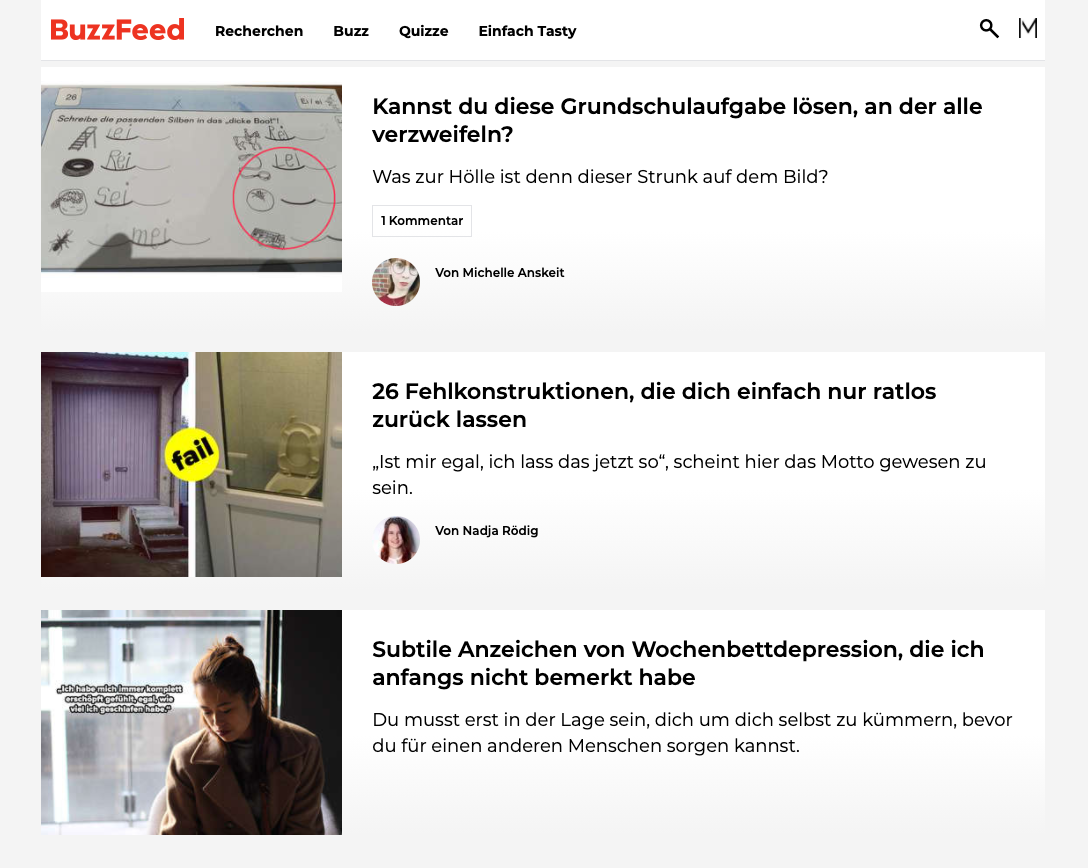
\includegraphics[width=11cm]{kapitel4/buzz.png}
    \caption[Beispiele von Clickbaits]{Beispiele von Clickbaits Nachrichten im Internet}
    \label{clckbPic}
\end{figure}

\begin{figure}[H]
    \centering
    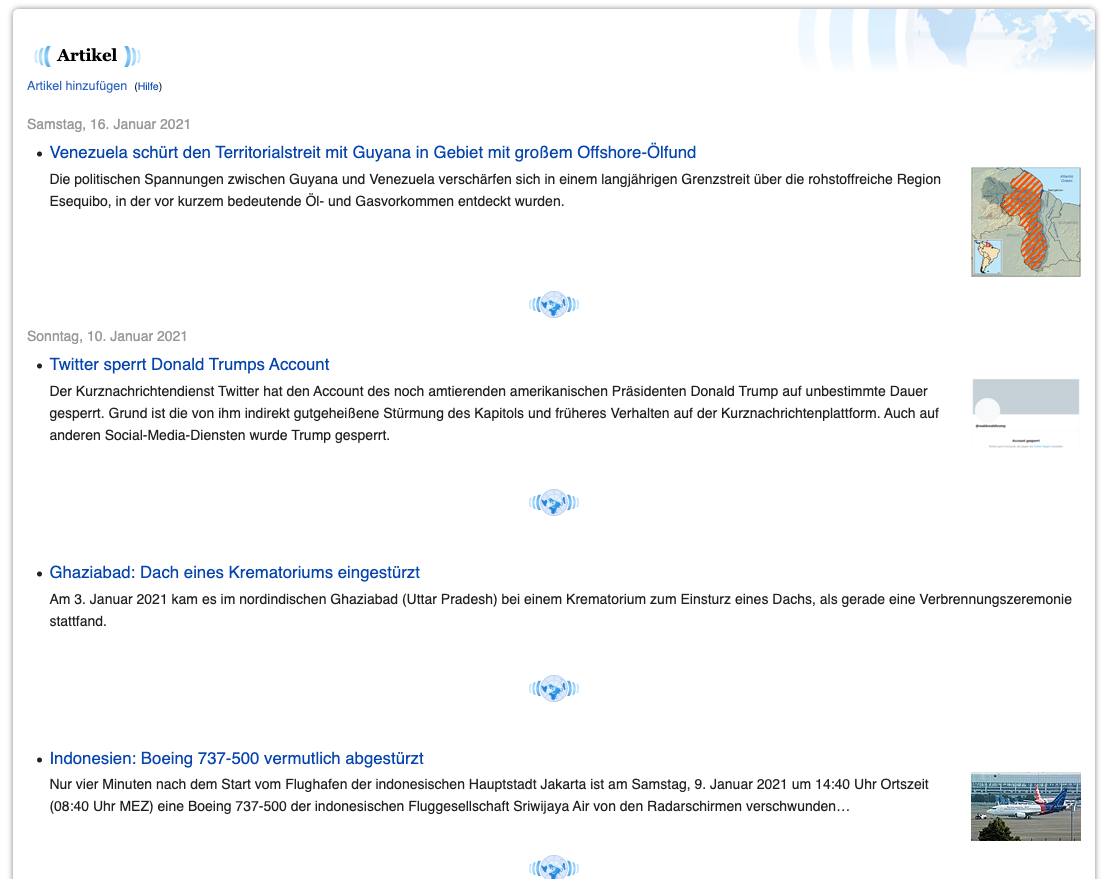
\includegraphics[width=11cm]{kapitel4/wikinews.png}
    \caption[Beispiele von Nicht-Clickbaits]{Beispiele von Nicht-Clickbaits Nachrichten im Internet}
    \label{clckbPic}
\end{figure}

Es gibt keine eindeutige Definition für Clickbaits. Clickbaits weisen unterschiedliche Formen. Nach \cite*{Biyani2016} sind Clickbaits, eine Praxis um Klicks zu generieren, durch eine attraktive Überschrift, wessen Inhalt die Erwartungen nur teilweise oder gar nicht erfüllt. Clickbaits können also als eine Täuschung oder Trick der Medien betrachtet werden. Eine andere Definition \cite*{Potthasta} betrachtet das Thema Clickbaits eher als Werbung für Onlineinhalte und die damit verbundene Verbreitung oder \enquote{Viral gehen} durch die sozialen Medien.

\begin{figure}[H]
    \centering
    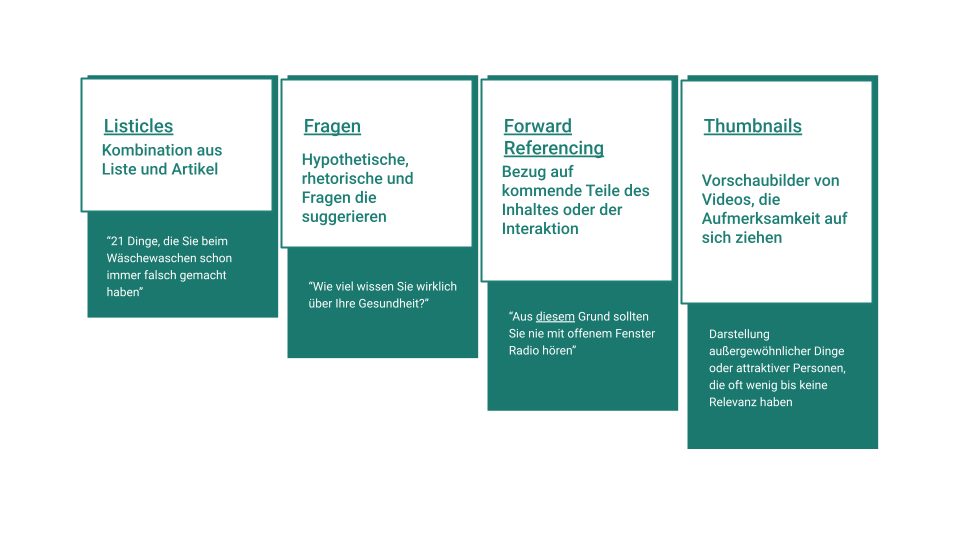
\includegraphics[width=15cm]{kapitel4/clickbaits.png}
    \caption[Die Kernformen des Clickbaits]{Die 4 Kernformen des Clickbaits in Anlehnung an \cite*[71]{Hrsg2020}}
    \label{TSNE}
\end{figure}

In \cite*[70-71]{Hrsg2020} werden Clickbaits in 4 Unterkategorien aufgeteilt. Der Autor bezieht sich dabei auf 4 Quellen und teilt Clickbaits als \textit{Listicles} \cite*{Vijgen2014}, \textit{Fragen} \cite*{Lai2014}, \textit{Forward Referencing} \cite*{Blom2015} und \textit{Thumbnails} \cite*{Zannettou2018} auf. Diese 4 Kategorien betrachtet der Autor als Kernkategorien. Aus \cite*[71]{Hrsg2020} werden Clickbaits außerdem in weitere Gestaltungsformen wie etwa, dass sie \enquote{Übertreibungen} sein können also falsche Versprechen geben oder irreführend sind und unklar sein können. Es wird außerdem auf die unangemessene und vulgäre Sprache und der Formatierung, wie etwa den übertriebenen Gebrauch von Großschreibung oder Satzzeichen, aufmerksam gemacht. Der Autor \cite*[75-76]{Hrsg2020} macht deutlich, dass Clickbaits kein neu eingesetztes Stilmittel im Journalismus seien. Schließlich verwendet der Autor den Begriff \enquote{Neugier} beim Leser. Leser wollen oftmals über Themen wie Tod, Gewalt, Sex und Prominente \cite*{Tenenboim2015} unterhalten werden. 

Fraglich ist also, ob diese Themen auch als Clickbait betrachtet werden können oder wo die Grenze liegt zwischen Medien die Unterhalten und Clickbaits. Es sollte schließlich einem Leser klar sein, dass bestimmte Nachrichten den Zweck der reinen Unterhaltung haben. Die Frage ob diese Art der Nachrichten Clickbait ist oder Unterhaltung sollte also nicht nur am Titel selbst, sondern auch im Zusammenhang mit dem Inhalt gemessen werden. Leider hat wohl jeder Mensch eine andere Erwartung, sodass eine solche Messung für jeden Unterschiedlich sein kann. 




\section{Wie werden Clickbaits klassifiziert?}

In diesem Abschnitt geht es darum, aus der Literatur die aktuelle Forschung im Zusammenhang mit der Klassifikation von Clickbaits zu ermitteln. Diese Analyse hat den Zweck bestimmte \enquote{Erfolgsmodelle} zu erkennen und von diesen evtl. in den späteren Teilen der Arbeit Gebrauch machen zu können.

In der Studie \cite*{Chakrabortya} wurde eine Browser-Erweiterung erstellt, welches Clickbaits erkennen soll. Es wurden umfangreiche Daten sowohl für Clickbaits als auch für Nicht-Clickbait-Kategorien gesammelt. Für die Nicht-Clickbaits-Kategorien wurden 18.513 Wikinews Artikeln gesammelt. Der Vorteil dieser Artikel ist, dass diese von einer Community erstellt werden und jeder Nachrichtenartikel vor der Veröffentlichung von der Community geprüft wird. Es gibt Stilrichtlinien, die eingehalten werden müssen. Um Clickbaits zu finden, haben die Autoren manuell aus Seiten wie \enquote{Buzzfeed} oder \enquote{Upworthy} ca. 8000 Titel gecrawlt. Um falsche Negative zu vermeiden (d. h. die Artikel in diesen Bereichen, bei denen es sich nicht um Clickbaits handelt), wurden sechs Freiwillige rekrutiert um die Überschriften zu labeln. Schließlich wurden 7500 Titel zu jeder der beiden Kategorien zugefügt und es stand ein Datensatz der Größe 15.000 Artikel zur Verfügung. Um Daten zu erfassen, können auch Soziale Medien wie Twitter herangezogen werden, wie im Beispiel von \cite*{Potthast}.



Laut \cite*{Chakrabortya} sind die herkömmlichen Nicht-Clickbait Schlagzeilen kürzer als Clickbait Schlagzeilen. Traditionelle Schlagzeilen enthalten in der Regel meistens Wörter, die sich auf bestimmte Personen und Orte beziehen, während die Funktionswörter (Nomen, Verben und Adjektive) den Lesern zur Interpretation aus dem Kontext überlassen bleiben. Es wird hier als Beispiel gegeben \enquote{Visa-Deal oder kein Migranten-Deal, Türkei warnt EU}. Hier sind die meisten Wörter Inhaltswörter, die die wichtigsten Erkenntnisse aus der Geschichte zusammenfassen, und es gibt nur sehr wenige Verbindungsfunktionswörter zwischen den Inhaltswörtern. Auf der anderen Seite sind Clickbait Schlagzeilen länger. Die Sätze, enthalten sowohl Inhalts- als auch Funktionswörter. Ein Beispiel für solche Schlagzeilen ist \enquote{Ein 22-Jähriger, dessen Ehemann und Baby von einem betrunkenen Fahrer getötet wurden, hat ein Facebook-Plädoyer veröffentlicht}. Obwohl die Anzahl der Wörter in Clickbait-Schlagzeilen höher ist, ist die durchschnittliche Wortlänge kürzer. Es werden häufig Wörter verwendet wie \enquote{Sie werden}, \enquote{Sie sind}. Im Durchschnitt haben die Wörter bei den Clickbaits längere Abhängigkeiten als Nicht-Clickbaits. Der Hauptgrund ist die Existenz komplexerer Phrasensätze im Vergleich zu Schlagzeilen ohne Clickbait. Es ist außerdem zu sehen, dass in Clickbait-Schlagzeilen Stoppwörter häufiger verwendet werden. Clickbait Überschriften verwenden häufig Determinantien wie \enquote{ihre}, \enquote{meine}, die auf bestimmte Personen oder Dinge im Artikel verweisen. Die Verwendung dieser Wörter trägt in erster Linie dazu bei, den Benutzer neugierig auf das Objekt zu machen, auf das verwiesen wird, und ihn zu überzeugen, den Artikel weiter zu verfolgen.


Um lexikalischer, semantische, orthografische und morphologische Merkmale zu erfassen, benutzen die Autoren aus \cite*{Anand2019} neben Worteinbettungen auch Zeicheneinbettungen.  Um Informationen außerhalb einzelner oder fester Wortfenster zu erfassen, untersuchten die Autoren dabei verschiedene RNN-Architekturen wie LSTM, GRU und Standard-RNNs. Dieses sind Wiederkehrende neuronale Netzwerkmodelle, die für sequentielle Daten wie Sprache und Text gut modelliert werden können.


Die Arbeit von \cite*{Agrawal2017} schlägt ein Modell vor, welches CNNs benutzt. CNNs werden für verschiedene Deep-Learning-Aufgaben verwendet. Es wurde hier nur eine Faltungsschicht in das CNN-Modell eingebaut. Die erste Schicht wird für das Einbetten der Wörter in Vektoren verwendet. Dabei wurden 2 verschiedene Worteinbettungen in Bezug genommen. Ein vortrainiertes und eines welches von Grund auf lernen musste und sich während des Trainings weiterentwickelt. In der nächsten Schicht werden Filter in verschiedenen Größen verwendet um Faltungen über Wortvektoren zu erzeugen.

Die Autoren der Arbeit aus \cite*{Pujahari} Clustern zunächst die aus den Schlagzeilen erstellten Vektoren mit der sogenannten t-SNE Methode nach \cite{VanDerMaaten2008}. Dieser Algorithmus rekategorisiert die Schlagzeilen in mehrere Gruppen und reduziert die vielen Dimensionen von Clickbaits im Datensatz. Die Autoren beginnen erst im nächsten Schritt mit dem Training. Dabei entstehen 11 Kategorien von Clickbaits (unter Anderem Kategorien wie \enquote{Mehrdeutig}, \enquote{Übertreibung} oder \enquote{Neckerei}).


\begin{figure}[H]
    \centering
    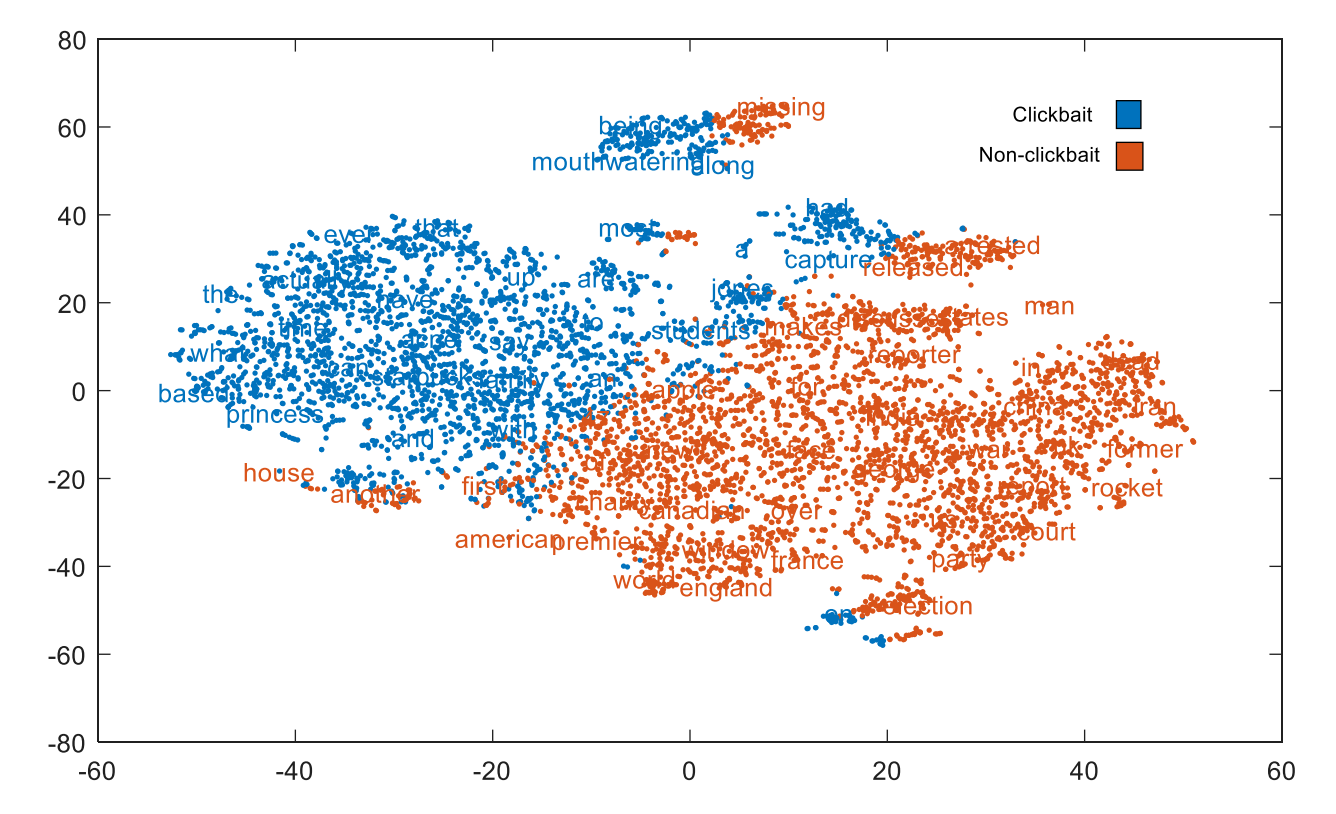
\includegraphics[width=12cm]{kapitel4/tsne.png}
    \caption[Clustering von Überschriften mit t-SNE]{Die Autoren verwenden das t-SNE Algorithmus nach \cite{VanDerMaaten2008} um die Dimensionen zu Reduzieren und es entstehen mehrere Unterkategorien von Clickbaits. Entnommen aus \cite*{Pujahari}.}
    \label{TSNE}
\end{figure}

